\documentclass[11pt]{article}
\usepackage[english]{babel}
\usepackage[T1]{fontenc}
\usepackage{amsmath}

% Graphic
\usepackage{caption}
\usepackage{subcaption}
\usepackage{graphicx}
\usepackage{xcolor}
\usepackage{geometry}
\geometry{
 a4paper,
 total={170mm,257mm},
 left=20mm,
 top=20mm,
}

% Math
\usepackage{algorithm}
\usepackage[noend]{algpseudocode}

% Links
\usepackage{hyperref}
\usepackage{url}

% Citing
\usepackage{apacite} 
\bibliographystyle{apacite}
\newcommand\shortcites[1]{\shortciteauthor{#1}'s\ \citeyear{#1}}



\title{\vspace{-0.8cm}Self-organisation of vowel systems in scale-free networks}
\author{Wolf De Wulf}
\date{}

\begin{document}
\maketitle

\begin{abstract}
    Simulations in agent-based systems that model populations of communicating agents have been used to show that due
    to
    interactions between these agents and self-organisation, realistic vowel systems emerge. Various independent
    studies
    have reported this phenomenon under various parameter configurations. The models used in these studies range from
    modelling only what is necessary to demonstrate emergence to modelling complex real life factors to investigate the
    impact on the emerged vowel repertoires. A common factor in a lot of these studies is the unrealistic assumption
    that
    every agent regularly communicates with every other agent. This article presents the analysis of a reimplementation
    of
    one of the first agent-based models that was created to analyse emergence in vowel systems. The model is extended
    to
    run simulations in scale-free networks. While scale-free networks are known to be rare in real life society, the
    simulations have allowed for gaining insights into the biases of the original system and into how it
    could be made to model society more accurately.
\end{abstract}

\section{Introduction}
It has been known for some time now that self-organisation through repeated interactions between people explains more
about the evolution of the sound systems of humans than innate predispositions do.
\shortciteA{liljencrantsNumericalSimulationVowel1972} showed that realistic vowel systems emerge when a measure of
energy, based on the statistics used by physicists, is optimised in an acoustic space of vowels. After
that,~\shortciteA{deboerSelforganizationVowelSystems2000} was the first to model a small population of agents that can
communicate with each other through a number of steps that are together deemed the `imitation game'. The agents
in~\shortcites{deboerSelforganizationVowelSystems2000} model had no innate predispositions and were still able to
converge to a global and realistic vowel system. Thereby showing that innate predispositions are not needed to explain
the evolution of vowel systems. However,~\shortcites{deboerSelforganizationVowelSystems2000} model contained a number
of ad hoc methods that could have been left out without influencing the results. Successing models such as those
by~\shortciteA{oudeyerSelfOrganizationSpeechSounds2005} and~\shortciteA{deboerMultiAgentSimulationsEvolution2010} did
so successfully while also investigating other questions such as whether or not agents should already possess the ability to imitate
and whether combinatorial structure emerges when instead of single vowels, sequences of vowels are
modelled. A common factor in the older models and even in most of the newer models is the assumption that every agent
regularly communicates with every other agent. In reality such fully connected networks are only found in very small
communities or in families. Therefore, these models might not capture dynamics that are present in large real life
populations. To address this, the model that is presented in this article
reimplements~\shortcites{deboerSelforganizationVowelSystems2000} model to run its simulations in a scale-free network.
The work that is presented here is very similar to that of~\shortciteA{ravivRoleSocialNetwork2020}, who investigated the role of social
network structure in the emergence of linguistic structure and also compared fully connected networks to scale-free networks.

Scale-free networks are networks whose degree distribution follows a power law. Such networks consist of two types of
nodes: nodes with a high degree called `hubs' and nodes with a small degree. While many real life networks were thought
to be scale-free, recent studies involving new rigorous statistical analysis techniques have showed that this is not
the case~\shortcite{clausetPowerLawDistributionsEmpirical2009,broidoScalefreeNetworksAre2019}. Examples of networks
that are thought to be scale-free are financial
networks~\shortcite{demasiFitnessModelItalian2006,soramakiTopologyInterbankPayment2007}, computer networks such as the
internet~\shortcite{faloutsosPowerlawRelationshipsInternet1999} and some social networks such as the co-authorship of
papers~\shortcite{newmanStructureScientificCollaboration2001}.
In the context of modelling a population, the idea of social networks following a scale-free structure is interesting.
Even though a network of, for example, co-authorship in mathematical papers is not one in which phonology plays an
important role, investigating what happens when an agent-based model that is designed to model a fully connected population of
communicating agents is adapted to run its simulations in such a network, should prove to be insightful. This is
exactly the case for the~\shortcites{deboerSelforganizationVowelSystems2000} model. The reimplementation of this model
that is presented in this article shows that emergence is different in scale-free populations.
While in fully connected populations, population size does not influence convergence, in scale-free populations this is not the case.
Insights into the influence of network structure on emergence are gained through a number of
experiments.

In what follows, Section~\ref{sec:SF} gives an in depth discussion on scale-free networks, the methods that can be used
to generate them and how they can be related to real life networks. Subsequently, Section~\ref{sec:methods} repeats the architecture
of~\shortcites{deboerSelforganizationVowelSystems2000} model and the adjustments that are made for it to run its
simulations in scale-free networks. Afterwards, Section~\ref{sec:exp} establishes a number of experiments of which
Section~\ref{sec:discus} discusses the results. Section~\ref{sec:conclusion} concludes the article with a number of
conclusions and possible future work.

\section{Scale-free networks\label{sec:SF}}
Scale-free networks are networks whose degree distribution asymptotically follows a power law. In a pure scale-free
network the probability of a node to have $k$ edges to other nodes is defined as follows:
\begin{align}
    P(k) \sim k^{-\gamma}
\end{align}
with $\gamma$ a scaling parameter typically in the range $2 \leq \gamma \leq 3$. Evidence for scale-free structure in a
network can be found using statistical techniques. \shortciteA{broidoScalefreeNetworksAre2019} summarise the different
notions of evidence in a set of categories which are not repeated here. For the rest of this article it suffices to
know that the used scale-free networks belong to the ``strongest'' category, which is due to the method that is used to
generate them. The scale-free networks in this article are generated using the most known mechanism to do so, called
preferential attachment~\shortcite{albertStatisticalMechanicsComplex2002}. The preferential attachment mechanism to
generate a scale-free network of size $N$ is given by Algorithm~\ref{alg:PA}.

\begin{algorithm}
    \caption{Preferential attachment \protect\shortcite{albertStatisticalMechanicsComplex2002}}\label{alg:PA}
    \begin{algorithmic}[1]
        \State $net \gets fully\_connected(4);$
        \While{$net.size() < N$}
        \State $A \gets net.new\_node();$
        \State $count \gets 4;$
        \While{$count != 0$}
        \State $B \gets net.random\_node();$
        \If{$!net.connected(A,B)$}
        \State $net.connect(A,B) \textbf{ with probability } \frac{B.degree}{net.total\_degree}$
        \EndIf
        \EndWhile
        \EndWhile
    \end{algorithmic}
\end{algorithm}
\noindent
The mechanism starts by initialising the network as a fully connected network of four nodes. Subsequently, the network
is expanded by adding nodes until the network consists of $N$ nodes. Each time a node is added, the following steps are
repeated 4 times: select a random node from the network, if the random node is not connected to the new node, connect
them with probability:
\begin{align*}
    P(k_i) = \frac{k_i}{\sum_{j} k_j}
\end{align*}
where $k_i$ is the degree of the randomly selected node. Hence, preferential attachment is a probabilistic mechanism.
New nodes are allowed to connect to any other node in the network. However, if a new node can be connected to a node
with degree 2 or to a node with degree 4, the node with degree 4 is twice as likely to be chosen.

Whether or not preferential attachment can be used to accurately describe a population of humans is a topic that has
sparked a lot of debate. Intuitively, the `hubs' created by the preferential attachment mechanism seem to be realistic.
By varying the scale and the context of the community a scale-free network is supposed to model, its adequacy varies as
well. Take, for example, a university community consisting of professors and students. In such a case, a scale-free
network seems like an adequate depiction of the underlying network. On the other hand, a much smaller community of
hunter-gatherers might be more accurately modelled by a fully connected network. By analysing a variety of real life
networks,~\shortciteA{broidoScalefreeNetworksAre2019} came to the conclusion that social networks are at best `weakly'
scale-free. Nevertheless, adapting models such as those of~\shortciteA{deboerSelforganizationVowelSystems2000}
and~\shortciteA{oudeyerSelfOrganizationSpeechSounds2005} to run their simulations in large and complex social networks
would result in incorrect representations of reality. When sound systems started emerging for the first time, social
networks were surely much smaller and simpler than those analysed by~\shortciteA{broidoScalefreeNetworksAre2019}.
Similarly to how language is said to be the result of the co-evolution of biological and cultural
inheritance~\shortcite{deboerBiologyCultureCoevolutionFinite2018}, the evolution of language and the structure of
society are two concurrent evolutionary processes that influence each other. Therefore, modelling an evolving sound
system in a fixed network structure is not realistic. A more realistic introduction of network structure into models
that investigate the emergence of sound systems would require network structure to evolve as well. This does not mean
that looking at what happens when a particular fixed network structure is added to a model that investigates the
emergence of vowel systems is entirely useless. While the speeds at which language and societal structure co-evolve are
likely to be much more comparable than those of biological and cultural inheritance, fixing network structure in a
model can still provide insights into one direction of the co-evolution, namely, the influence of network structure on
the evolution of language.

\section{Methodology\label{sec:methods}}
Aside from two changes, the model\footnote{The source code of the model can be found on GitHub:
    \url{https://github.com/wulfdewolf/ProjectEoS}} that is presented here is exactly the same as that
of~\shortciteA{deboerSelforganizationVowelSystems2000}. Originally, the model was implemented in $C$++ and while this did
not change, the model was reimplemented for compatibility reasons. The two aspects that were adapted in  the first
model are the following: the network architecture in which the simulations run and the bark-to-hertz and hertz-to-bark
conversions.

Figure~\ref{fig:model} gives a graphical representation of the steps that are executed during a simulation. Every agent A is separately chosen
to be the \textit{sender} of the iteration. With a certain probability, agent $A$ is allowed to add a new distributed vowel to their repertoire.
The distribution of vowels is implemented just as it was by~\shortciteA{deboerSelforganizationVowelSystems2000}: by
maximising the distance to all other vowels. Subsequently, every agent merges its vowels that are too alike until no merges
are possible. The merging threshold is $0.17$ in articulatory space and $\frac{log(1+noise)}{0.1719} - \frac{log(1-noise}{0.1719}$, in acoustic space.
\shortciteA{deboerSelforganizationVowelSystems2000} defines these values to be the maximum distance a vowel can be shifted by ambient noise.
After merging, a random neighbour $B$ of agent $A$ is chosen to be the receiver of the iteration.
Originally,~\shortciteA{deboerSelforganizationVowelSystems2000} chose the receiver agent as a random agent from the
complete population, thereby modelling a fully connected network. Once a sender and a receiver have been chosen, an
imitation game is played. Agent $A$ chooses a random vowel $v_A$ from their repertoire, synthesises it, and sends it to
agent $B$ as an utterance $v'_A$, thereby adding a noise shift. If agent $A$'s repertoire was empty, it is
initialised with a completely random vowel. Agent $B$ hears the synthesised vowel $v'_A$ and finds the most resembling
vowel $v_B$ in their repertoire, synthesises it, and sends it to agent $A$ as an utterance $v'_B$, once more, adding a
noise shift. Agent $A$ hears agent $B$'s response and finds the most resembling vowel in their repertoire. If
this vowel is the original $v_A$ then the imitation game was successful and agent $A$ sends \textit{True} to agent $B$,
otherwise the imitation game failed and agent $A$ sends \textit{False} to agent $B$. Lastly, agent $B$ receives the
success boolean and does the following. If it is \textit{True}, agent $B$ moves $v_B$ closer to $v_A$, since by
uttering $v_B$ agent $A$ was able to understand agent $B$. If it is \textit{False} and the success rate of $v_B$ is $>\beta_S$ (soft success threshold)
then agent $B$ moves $v_B$ away from $v_A$ and adds a new vowel as close as possible to $v_A$. The reasoning
behind this is that $v_B$ is not a bad vowel because it is successful to some degree. It is rather that
agent $A$ probably has another vowel that is closer to $v_B$ than $v_A$ is. Therefore, agent $B$ should learn this
vowel. If the received boolean is \textit{False} and the success rate of $v_B$ is $\leq \beta_S$, then agent $B$ still
moves $v_B$ closer to $v_A$, however, this does not add to the success rate of $v_B$. Finally, after the imitation game
and with probability $\alpha$, every agent is allowed to remove the bad vowels from their repertoires.
Vowels that have been used at least 5 times and have a success rate $< \beta_H$ (hard success threshold) are removed. As mentioned, the network
that determines an agent's neighbours is generated using Algorithm~\ref{alg:PA}. Synthesising, shifting vowels and
distance measures are all implemented as they were by~\shortciteA{deboerSelforganizationVowelSystems2000}.

\begin{figure}[t]
    \centering
    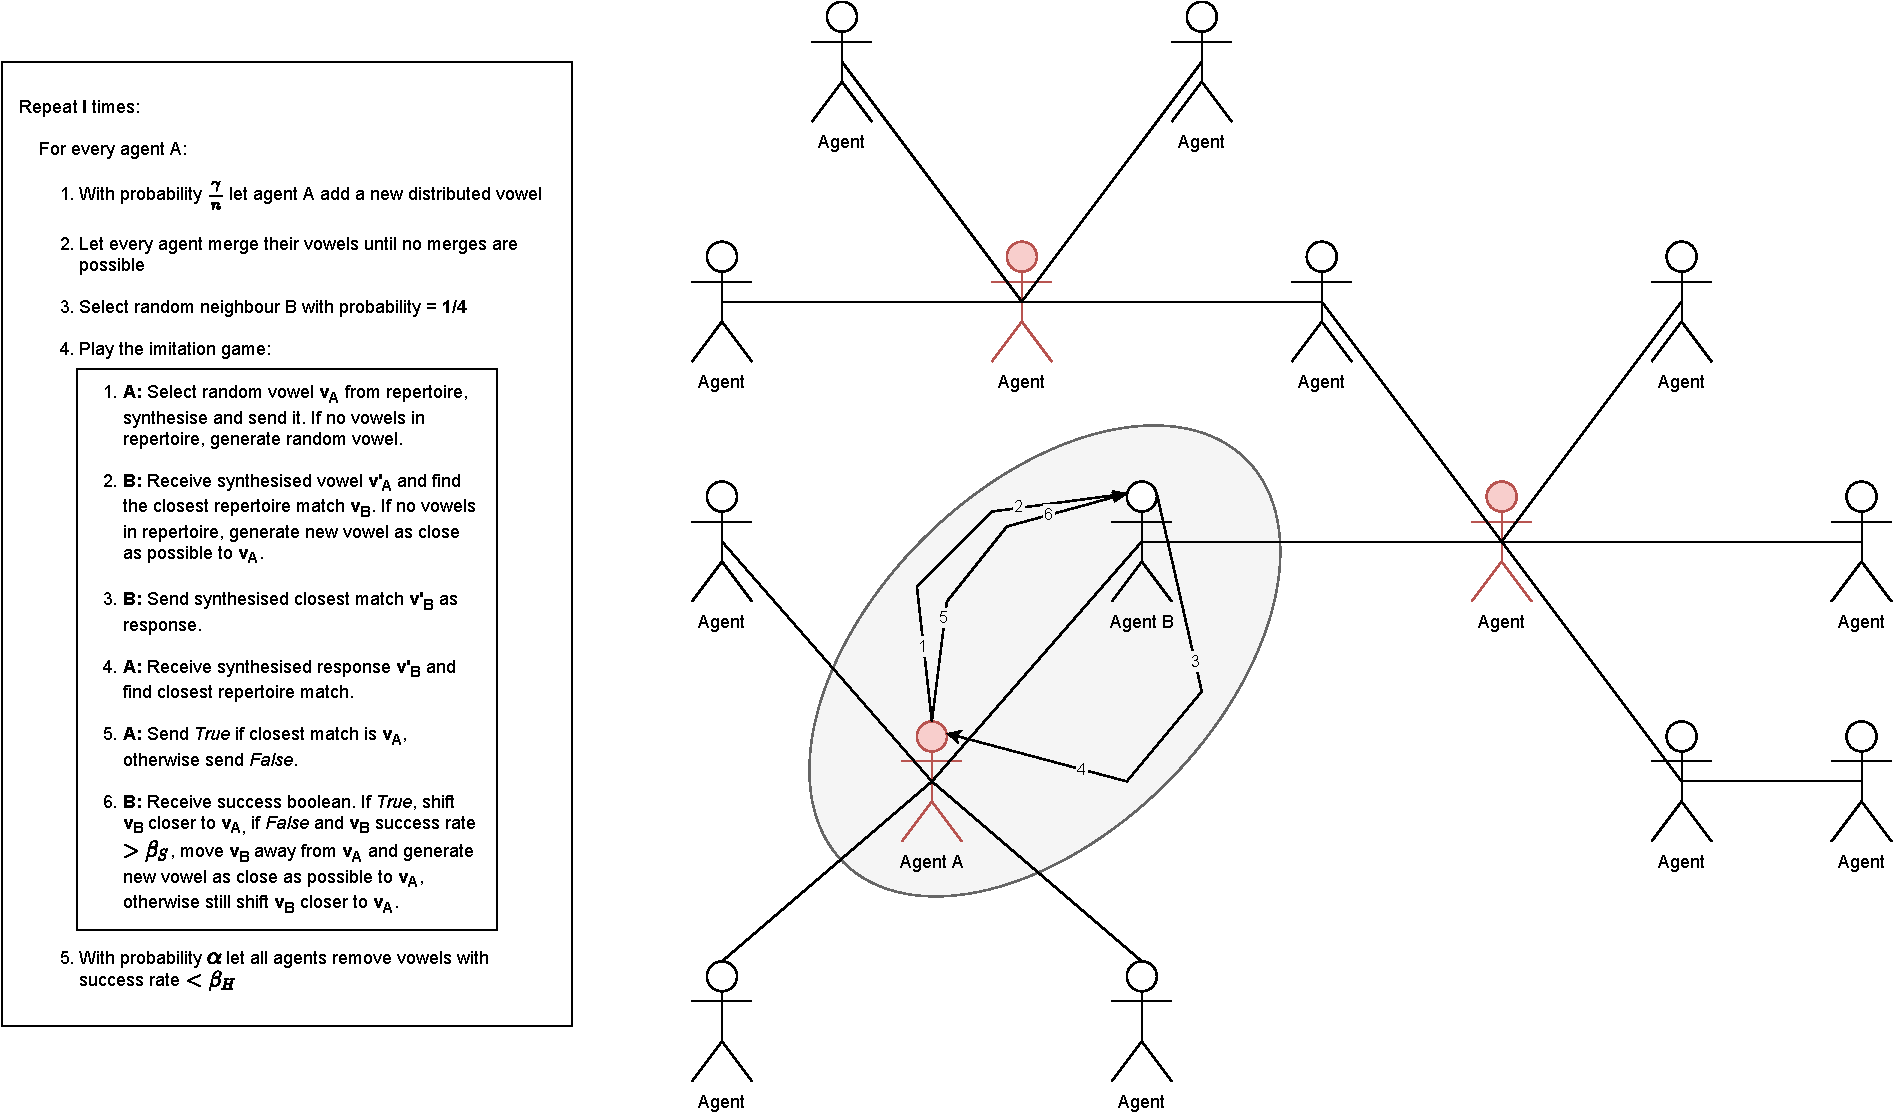
\includegraphics[width=\textwidth]{figures/simulation_diagram.pdf}
    \caption{Graphical representation of the steps that are executed during a simulation.}
    \label{fig:model}
\end{figure}

The bark-to-hertz and hertz-to-bark conversions that were implemented
by~\shortciteA{deboerSelforganizationVowelSystems2000} are interpolations based on data from other papers. The second
adaptation to~\shortcites{deboerSelforganizationVowelSystems2000} model is the implementation of the conversions that
are implemented in
MATLAB\footnote{\url{https://nl.mathworks.com/help/audio/ref/bark2hz.html}}\footnote{\url{https://nl.mathworks.com/help
        /audio/ref/hz2bark.html}}, which are based on the work
of~\shortciteA{traunmullerAnalyticalExpressionsTonotopic1990}:
\begin{align}
    bark & = \begin{cases}
        \frac{bark - 0.3}{0.85}   & \text{ if } bark < 2    \\
        \frac{bark + 4.422}{1.22} & \text{ if } bark > 20.1 \\
        bark                      & \text{ otherwise}
    \end{cases}
\end{align}
and:
\begin{align}
    bark & = \frac{26.81 * hertz}{1960 + hertz} - 0.53 \\
    bark & = \begin{cases}
        bark + 0.15 * (2- bark)     & \text{ if } bark < 2    \\
        bark + 0.22 * (bark - 20.1) & \text{ if } bark > 20.1 \\
        bark                        & \text{ otherwise}
    \end{cases}
\end{align}
While different conversions will most likely not change much in the results, for comparability it is better to use some
standardized implementation.

\section{Experiments\label{sec:exp}}
Three experiments are conducted. Firstly, the experiment from Section 4.1
from~\shortcite{deboerSelforganizationVowelSystems2000} is reproduced for the fully connected model. This serves to demonstrate that the
reimplementation of the model is correct. Secondly, said experiment is also conducted for an instance of the model that runs its
simulations in a scale-free network. By comparing the results of the two, insights can be gained regarding the research question that
is addressed here. Lastly, one of the experiments from Section 4.2 from~\shortcite{deboerSelforganizationVowelSystems2000} is reproduced for
the scale-free model. Namely, the experiment that investigates the influence of the population size on the emergence.
Due to the difference in network structure it is reasonable to expect different results for this experiment.

An adaptation to the simulations of~\shortciteA{deboerSelforganizationVowelSystems2000} that is
implemented here is that the number of played imitation games is always kept per agent and never globally.
While~\shortciteA{deboerSelforganizationVowelSystems2000} only implemented this to allow for correct comparisons
between the results of simulations with different population sizes, here it is implemented for all the experiments, solely for practicality.
In addition, to allow for correct comparisons when population sizes are varied, the probability of adding new distributed vowels must be made dependent on the
number of imitation games played per agent instead of on the global number of played imitation games. Therefore,~\shortciteA{deboerSelforganizationVowelSystems2000}
sets the probability of adding new distributed vowels to $\frac{\gamma}{N}$, with $N$ the population size and $\gamma$ a parameter.
\shortciteA{deboerSelforganizationVowelSystems2000} chose $\gamma=0.2$ such that for a population of 20 agents the insertion probability is $1\%$.
In all simulations that are presented here, the same formula and $\gamma$ are used.

Aside from the population size and $\gamma$, the model has a variety of other parameters (values taken from \shortcite{deboerSelforganizationVowelSystems2000}): the probability of letting agents
remove bad vowels $\alpha=0.1$, the relative weight of the effective second formant with respect to the first formant $\lambda=0.3$, the acoustic noise $\sigma=0.1$, the soft vowel success
threshold $\beta_S=0.5$, and the hard vowel success threshold $\beta_H=0.7$.
Aside from the population size in the third experiment, all of these remain constant in all experiments.

\shortciteA{deboerSelforganizationVowelSystems2000} evaluates the robustness of
the results by repeating the simulations 1000 times and plotting the success, size, and energy distributions.
The energy of an agent's repertoire is calculated using the energy measure defined by~\shortciteA{liljencrantsNumericalSimulationVowel1972}:
\begin{align}
    \label{form:energy}
    E = \sum^{N-1}_{i=1}\sum^{i-1}_{j=0} \frac{1}{r_{ij}^2}
\end{align}
with $r_{ij}$ the distance between vowels $i$ and $j$.
This is all repeated here as well.

\section{Discussion\label{sec:discus}}

\begin{figure}[t]
    \centering
    \subcaptionbox[Short Subcaption]{%
        Fully connected%
        \label{subfig:FC_res}%
    }
    [%
        \textwidth % width of caption
    ]%
    {%
        \includegraphics[scale=0.23]{figures/plots/exp1/FC/1.pdf}
        \includegraphics[scale=0.23]{figures/plots/exp1/FC/25.pdf}
        \includegraphics[scale=0.23]{figures/plots/exp1/FC/100.pdf}
        \includegraphics[scale=0.23]{figures/plots/exp1/FC/500.pdf}
    }%
    \\\bigskip
    \subcaptionbox[Short Subcaption]{%
        Scale-free%
        \label{subfig:BA_res}%
    }
    [%
        \textwidth % width of caption
    ]%
    {%
        \includegraphics[scale=0.23]{figures/plots/exp1/BA/1.pdf}
        \includegraphics[scale=0.23]{figures/plots/exp1/BA/25.pdf}
        \includegraphics[scale=0.23]{figures/plots/exp1/BA/100.pdf}
        \includegraphics[scale=0.23]{figures/plots/exp1/BA/500.pdf}
    }%
    \caption{Combined vowel repertoires of a population of 20 agents after 1, 25, 100, and 500
        imitation games per agent.}
    \label{fig:res}
\end{figure}

\subsection{Emergence of a vowel system}
Figure~\ref{subfig:FC_res} gives the emergence of a vowel system in a fully connected population of 20 agents under $10\%$ acoustic noise.
The prototypes of the agents' vowels are combined and plotted in the $F_1-F'_2$ space. The combined repertoires are shown after 1, 25, 100 and 500 games per agent.
After 1 imitation game per agent it can be seen that the vowels are distributed across the vowel space. There is already some tendency to cluster.
This corresponds to the results in~\shortcite{deboerSelforganizationVowelSystems2000} and is due to the fact that agents start out with an empty repertoire and
random vowels are inserted to get the imitation games started. The receiver agents try to imitate utterances as good as possible and this causes the early clusters.
After 25 imitation games per agent, the clustering has become more pronounced, two to three clusters seem to form. At this point clusters will start compacting.
However, there still seem to be only two to three clusters and the vowel space has space for extra vowels.
After 100 imitation games per agent, some clusters have become more compact and the vowel space has become more filled.
Lastly, after 500 games per agent, the clusters are all tightly packed and some additional clusters have been established.
At this point, the vowel system is stable to some degree. New clusters can still be formed and the existing clusters move around but generally the vowel system remains the same.
These results correspond to those of~\shortciteA{deboerSelforganizationVowelSystems2000}.

Figure~\ref{subfig:BA_res} depicts the same results but for the scale-free model.
While the situations after 1, 25, and 100 imitation games seem to roughly correspond to those of the fully connected model, after 500 imitation games, the clusters still seem
to struggle to become compact. Even after 500 imitation games per agent some of the clusters still consist of subclusters.
This can surely be a result of the scale-free architecture of the population.
The hubs that a scale-free network contains make compacting the clusters more difficult.
A hypothesis for the cause of this is that intra-hub communication can keep a hub-specific variant of a vowel in tact in such a way that inter-hub
communication using this vowel is still succesful. Such a phenomenon would model the existence of dialects in the real world.
However, more experiments need to be conducted to verify such an hypothesis.
Aside from the non-perfectly compacted clusters, the results for a scale-free population seem to correspond to the results for a fully connected population.
This matches with the results of~\shortciteA{ravivRoleSocialNetwork2020}.

\begin{figure}[t]
    \centering
    \subcaptionbox[Short Subcaption]{%
        Fully connected%
        \label{subfig:FC_stats}%
    }
    [%
        \textwidth % width of caption
    ]%
    {%
        \includegraphics[scale=0.3]{figures/plots/exp1/FC/success_distribution.pdf}
        \hfill
        \includegraphics[scale=0.3]{figures/plots/exp1/FC/size_distribution.pdf}
        \hfill
        \includegraphics[scale=0.3]{figures/plots/exp1/FC/energy_distribution.pdf}
    }%
    \\\bigskip
    \subcaptionbox[Short Subcaption]{%
        Scale-free%
        \label{subfig:BA_stats}%
    }
    [%
        \textwidth % width of caption
    ]%
    {%
        \includegraphics[scale=0.3]{figures/plots/exp1/BA/success_distribution.pdf}
        \hfill
        \includegraphics[scale=0.3]{figures/plots/exp1/BA/size_distribution.pdf}
        \hfill
        \includegraphics[scale=0.3]{figures/plots/exp1/BA/energy_distribution.pdf}
    }
    \caption{Distribution of statistics for 1000 simulations in a population of 20 agents after 500 imitation games
        per agent.}
    \label{fig:stats}
\end{figure}

\subsection{Evaluation of the emerged vowel systems}
To verify if the vowel systems that emerge are realistic,~\shortciteA{deboerSelforganizationVowelSystems2000} analyses three properties: the average size of the agents'
vowel systems, the average number of succesful imitation games, and the energy as defined by~\shortciteA{liljencrantsNumericalSimulationVowel1972} and given by~(\ref{form:energy}).
\shortciteA{liljencrantsNumericalSimulationVowel1972} showed that minimising their energy function results in realistic vowel systems.~\shortciteA{deboerSelforganizationVowelSystems2000}
therefore choses to consider vowel systems with near-minimal energy to be realistic, this is done here as well.
In a second verification,~\shortciteA{deboerSelforganizationVowelSystems2000} compares the emerged vowel systems to real life vowel systems, this is not repeated here.

Figure~\ref{subfig:FC_stats} shows the distributions of the three measures for a fully connected population, these results were obtained by averaging of 1000 simulations of 500 imitation games per
agent each. The average success is always very high, it ranges between 0.90 and 1.00 and the distribution is skewed to the left. The size distribution shows various average repertoire sizes and clear
peaks at integer values of the sizes 6 to 8. This is because the population's agents tend to have the same number of vowels in their repertoires. Therefore, the vowel systems that emerged can be
assumed to be uniform among all agents. However, the simulations did not always end with a vowel system of the same size. In addition, there is an obvious peak for vowel systems that
contain 7 vowels. Just as in~\shortcite{deboerSelforganizationVowelSystems2000}, this can be changed by increasing or decreasing the noise.
Lastly, the energy distribution shows peaks as well. These correspond to the different sizes of vowel systems and to their different configurations. The distribution is very similar to that of
\shortciteA{deboerSelforganizationVowelSystems2000} and thus the emerged vowel systems can be asumed to be optimal and, in some way, realistic.
In general, the results correspond to those of~\shortciteA{deboerSelforganizationVowelSystems2000}.

Figure~\ref{subfig:BA_stats} shows the distributions of the three measures for a scale-free population.
Consistent with the results of the previous sections, the same observations can be made. This also matches with the results
of~\shortciteA{ravivRoleSocialNetwork2020}.

\begin{figure}[t]
    \centering
    \subcaptionbox[Short Subcaption]{%
        20 agents%
        \label{subfig:BA_res20}%
    }
    [%
        \textwidth % width of caption
    ]%
    {%
        \includegraphics[scale=0.23]{figures/plots/exp1/BA/1.pdf}
        \includegraphics[scale=0.23]{figures/plots/exp1/BA/25.pdf}
        \includegraphics[scale=0.23]{figures/plots/exp1/BA/100.pdf}
        \includegraphics[scale=0.23]{figures/plots/exp1/BA/500.pdf}
    }%
    \\\bigskip
    \subcaptionbox[Short Subcaption]{%
        100 agents%
        \label{subfig:BA_res100}%
    }
    [%
        \textwidth % width of caption
    ]%
    {%
        \includegraphics[scale=0.23]{figures/plots/exp2/50/1.pdf}
        \includegraphics[scale=0.23]{figures/plots/exp2/50/25.pdf}
        \includegraphics[scale=0.23]{figures/plots/exp2/50/100.pdf}
        \includegraphics[scale=0.23]{figures/plots/exp2/50/500.pdf}
    }%
    \\\bigskip
    \subcaptionbox[Short Subcaption]{%
        300 agents%
        \label{subfig:BA_res300}%
    }
    [%
        \textwidth % width of caption
    ]%
    {%
        \includegraphics[scale=0.23]{figures/plots/exp2/100/1.pdf}
        \includegraphics[scale=0.23]{figures/plots/exp2/100/25.pdf}
        \includegraphics[scale=0.23]{figures/plots/exp2/100/100.pdf}
        \includegraphics[scale=0.23]{figures/plots/exp2/100/500.pdf}
    }%
    \caption{Combined vowel repertoires of a scale-free population of various sizes after 1, 25, 100, and 500
        imitation games per agent.}
    \label{fig:res_2}
\end{figure}

\begin{table}[b]
    \resizebox{\textwidth}{!}{%
        \begin{tabular}{|c|c|c|c|}
            \hline
            \textbf{Population size} & \textbf{Success distribution} & \textbf{Size distribution} & \textbf{Energy distribution} \\ \hline
            20                       & 0.9643 $\pm$ 0.01298          & 7.2685 $\pm$ 0.7670        & 4.4003 $\pm$ 1.0709          \\ \hline
            50                       & 0.9523 $\pm$ 0.01654          & 7.2133 $\pm$ 0.7047        & 4.2063 $\pm$ 0.8989          \\ \hline
            100                      & 0.9441 $\pm$ 0.01667          & 7.2474 $\pm$ 0.6507        & 4.1898 $\pm$ 0.7973          \\ \hline
        \end{tabular}%
    }
    \caption{Distribution of statistics for 1000 simulations in a scale-free population of various sizes after 500 imitation games
        per agent.}
    \label{tab:stats_2}
\end{table}

\subsection{Sensitivity to population size}
Figure~\ref{fig:res_2} gives the emergence of vowel systems in a scale-free population of 20, 50, and 100 agents under $10\%$ acoustic noise.
Accompanying it is Table~\ref{tab:stats_2}, which gives the parameters of the distributions of the three measures averaged over 1000 simulations, 500 imitation
games per agent each. Three observations can be made here. Firstly, the random dispersion of the vowels after 1 imitation game per agent in the population of 100
agents gives a good sketch of the form of the vowel space. Secondly, in the plots for the larger populations, almost line-like patterns show.
These can be accounted to the discrete steps that are taken when agents move vowels closer to another vowel. The implementation of this process was taken
from~\shortciteA{deboerSelforganizationVowelSystems2000} and consists of generating a number of neighbouring articulatory configurations, synthesising them and selecting the one
that is closest to the target vowel. Lastly, and most importantly, the larger populations seem to not be able to converge after 500 imitation games per agent.
The success, size, and energy distributions show interesting results. For the populations of 50 and 100 agents, the average repertoire size was found to also peak at non-integer values, hence, the
larger the population, the harder it is for the model to converge to a population where every agent has the same vowel repertoire.
This seems to also be reflected by the success and energy distributions, they seem to lie lower than those of the smaller population.
However, for both the population of 50 and 100 agents, according to the Kolmogorov-Smirnov test, this is only significant for the success distributions ($p<0.01$ for both).
This constrasts with what~\shortciteA{deboerSelforganizationVowelSystems2000} found for fully connected populations.
In such populations, the success statistic is comparable for different population sizes and the repertoire size was found to grow with the population size.
For scale-free populations this seems to not be the case. Intuitively, this is logical. The larger a scale-free population is, the more thightly intra-connected hubs exist, but the smaller
the probability of inter-hub communication becomes. Therefore, it becomes much more difficult to propagate vowels through out the network.
This matches the results of~\shortciteA{ravivLargerCommunitiesCreate2019}.
In some way this is realistic, because if it were otherwise, there would probably only exist one universal language in the world.

\section{Conclusions\label{sec:conclusion}}
A reimplementation of the model of~\shortciteA{deboerSelforganizationVowelSystems2000} that implements a scale-free network is presented.
Through a number of experiments it was found that for smaller populations, the models are similar. However, in larger populations it becomes more
difficult for the scale-free model to converge. It was shown that scale-free structure in a population makes it more difficult for the population to agree on a single sound system.

As a follow-up to this study, various different network architectures could be implemented to verify their influence on convergence. Particularly interesting could be to hand-tailor
network architectures to specific communities~\shortcite{willCombiningSocialNetwork2020}. Additionally, adding a dynamic aspect to the network structure should be interesting as
well~\shortcite{skyrmsDynamicModelSocial2000,sekaraFundamentalStructuresDynamic2016}.
Lastly, while the results here matched those of~\shortciteA{ravivRoleSocialNetwork2020} and~\shortciteA{ravivLargerCommunitiesCreate2019}, the emphasis of these articles lies on the
\textit{systematicity} of the emerged languages in different network architectures. Analysing the systematicity of vowel systems such as those used in this article might be difficult as the vowels
are
only used in a hollistic way. However, it might be interesting to do so using models that allow for combinatorial structure such as those of~\shortciteA{deboerMultiAgentSimulationsEvolution2010}.

\bibliography{refs}
\end{document}